
    \begin{align}
        Maximize : 3x_1 + 2x_2 \\
        Subject-to:
        x_1 + 2x_2  \leq 10 \\
        3x_1 + x_2 \leq 15 
    \end{align}
    The Problem is converted into canonical form by adding slack variables.Then Problem becomes,\\
    \begin{align}
        Maximize : 3x_1 + 2x_2 + 0s_1 + 0s_2\\
        Constraints :
        x_1 + 2x_2 + s_1 = 10 \\
        3x_1 + x_2 + s_2 = 15 
    \end{align}
        
    we write the Simplex tableau , \\
    \begin{align}
    \myvec{
    x_1 & x_2 & s_1 & s_2 & c \\[0.1cm]
    1 & 2  & 1 & 0 & 10 \\
    \hlight{3} & 1 & 0 & 1 & 15\\ \hline
    -3 & -2 & 0 & 0 & 0
    }
    \end{align}
    Keeping the Pivot element as $3$  and by using gauss-jordan Elimination we get \\
    \begin{align}
    \myvec{
    x_1 & x_2 & s_1 & s_2 & c \\[0.1cm]
    0 & \hlight{\frac{5}{3}}  & 1 & \frac{-1}{3} & 5 \\[0.1cm]
    1 & \frac{1}{3} & 0 & \frac{1}{3} & 5  \\[0.1cm] \hline
    0 & -1   & 0 & 1 & 15
    }
    \end{align}
    Keeping the Pivot element as $\frac{5}{3}$  and by using gauss-jordan Elimination we get \\
    \begin{align}
    \myvec{
    x_1 & x_2 & s_1 & s_2 & c \\[0.1cm]
    0 & 1  & \frac{3}{5} & \frac{-1}{5} & 2 \\[0.1cm]
    1 & 0 & \frac{-1}{5} & \frac{2}{5} & 3\\[0.1cm] \hline
    0 & 0   & \frac{3}{5} & \frac{4}{5} & 18
    }
    \end{align}
    In this tableau Since all  indicators in last row are non-negative ,we found optimal  solution to given problem.
    Therefore  Optimal Solution will be: \\
    \begin{align}
        (x_1,x_2) &= (4,3) \\
        Z &= 3x_1+2x_2 \\
        Z &= 3 \times 4 + 2 \times 3 \\
        Z &= 18
    \end{align}
    \begin{figure}[h]
    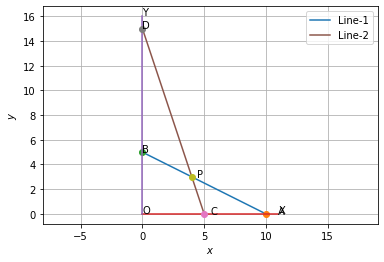
\includegraphics[width=\columnwidth]{./solutions/4/7/Figure_1.png}
    \caption{Region OBPC is Valid region}
    \label{eq:solutions/4/7/fig:Figure_1}
    \end{figure}\\
    
    This Problem can be represented in matrix form as follows,\\
    \begin{align}
        \max_{\vec{x}} Z &= \myvec{3 & 2}\vec{x}\\
        s.t. \quad 
        \myvec{
        1 & 2\\
        3 & 1
        }
        \vec{x} &\preceq \myvec{10\\15} \\
        \vec{x} &\succeq \vec{0}\\
        \vec{y} &\succeq \vec{0}
    \end{align}
    
    this is solved using cvxpy in python,we get \\
    \begin{align}
    \vec{x} = \myvec{3.99999999\\2.99999999}, Z = 17.99999996
    \end{align}

